% Chapter Template

\chapter{Technologies, Toolchain and Hardware} % Main chapter title

\label{Technologies, Toolchain and Hardware} % Change X to a consecutive number; for referencing this chapter elsewhere, use \ref{ChapterX}

%----------------------------------------------------------------------------------------
%	Hardware, Technologies, Toolchain and Programming Languages
%----------------------------------------------------------------------------------------

\section{Technologies and Programming Languages}

The software has three parts the backend, the frontend and the daemon, they communicate with each other throw a REST api[\footnote{\href{https://en.wikipedia.org/wiki/Representational\_state\_transfer}{\texttt{https://en.wikipedia.org/wiki/Representational\_state\_transfer}}}] (Figure \ref{fig:iothcomponentdiagram5}). So I will present them separately.
\newline

In software engineering, the terms "front end" and "back end" are distinctions which refer to the separation of concerns between a presentation layer and a data access layer respectively.
\newline

The front end is an interface between the user and the back end. The front and back ends may be distributed amongst one or more systems.
\newline

In software architecture, there may be many layers between the hardware and end user. Each can be spoken of as having a front end and a back end. The front is an abstraction, simplifying the underlying component by providing a user-friendly interface.
\newline

In software design, for example, the model-view-controller architecture provides front and back ends for the database, the user and the data processing components. The separation of software systems into front and back ends simplifies development and separates maintenance. A rule of thumb is that the front (or "client") side is any component manipulated by the user. The server-side (or "back end") code resides on the server. The confusion arises when one must make front-end edits to server-side files. Most HTML designers, for instance, don't need to be on the server when they are developing the HTML; conversely, the server-side engineers are, by definition, never on anything but a server. It takes both to ultimately make a functioning, interactive website.

\begin{figure}[h]
	\centering
	\includegraphics[width=0.7\linewidth]{uml/iothcomponent}
	\caption{Iot Healthcare: Component Diagram}
	\label{fig:iothcomponentdiagram5}
\end{figure}

\subsection{Backend}

The backend is a java application the main framework is Spring[\footnote{\href{https://spring.io/}{\texttt{https://spring.io/}}}].
Why Spring? First of all the development progress is really fast with Spring and this is a main reason, a second one will be my experience with spring because I start using Spring at work a few years ago and a third reason  spring is well integrated with the build system from Heroku instance.
\newline

The build system of the backend is Gradle[\footnote{\href{https://gradle.org/}{\texttt{https://gradle.org/}}}]. In the end the backend and the frontend they run in the same web container which is a Apache Tomcat[\footnote{\href{https://tomcat.apache.org/}{\texttt{https://tomcat.apache.org/}}}].
\newline

For the persistence layer I used Hibernate[\footnote{\href{http://hibernate.org/}{\texttt{http://hibernate.org/}}}] and JpaRepository[\footnote{\href{http://docs.spring.io/spring-data/jpa/docs/current/api/org/springframework/data/jpa/repository/JpaRepository.html}{\texttt{JpaRepository}}}] from Spring Framework.
\newline

The database is postgreSQL.[\footnote{\href{https://www.postgresql.org/}{\texttt{https://www.postgresql.org/}}}]. I chose postgreSQL because has JSON support and I know in the future I will switch to a schema-less for storing the activity of a patient and was also free in the Heroku instance.


%\begin{figure}[h]
%	\centering
%	\begin{minipage}{.5\textwidth}
%		\centering
%		
\includegraphics[width=.4\linewidth]{images/spring-logo}
%		\captionof{figure}{Spring}
%		\label{fig:springlogo}
%	\end{minipage}%
%	\begin{minipage}{.5\textwidth}
%		\centering
%		
\includegraphics[width=.4\linewidth]{images/postgresql-logo}
%		\captionof{figure}{postgreSQL}
%		\label{fig:postgre-logo}
%	\end{minipage}
%	\begin{minipage}{.5\textwidth}
%		\centering
%		
\includegraphics[width=.5\linewidth]{images/gradlephant}
%		\captionof{figure}{Gradle}
%		\label{fig:gradle-logo}
%	\end{minipage}%
%	\begin{minipage}{.5\textwidth}
%		\centering
%		\includegraphics[width=.5\linewidth]{images/Hibernate}
%		\captionof{figure}{Hibernate}
%		\label{fig:hibernate-logo}
%	\end{minipage}
%	\begin{minipage}{.5\textwidth}
%		\centering
%		
\includegraphics[width=.5\linewidth]{images/tomcat}
%		\captionof{figure}{Apache Tomcat}
%		\label{fig:tomcat-logo}
%	\end{minipage}
%\end{figure}


\subsection{Frontend}
The frontend is a web application, is based on the classic web technologies: HTML5[\footnote{\href{https://en.wikipedia.org/wiki/HTML5}{\texttt{https://en.wikipedia.org/wiki/HTML5}}}], CSS3[\footnote{\href{https://en.wikipedia.org/wiki/Cascading\_Style\_Sheets}{\texttt{https://en.wikipedia.org/wiki/Cascading\_Style\_Sheets}}}] and JavaScript[\footnote{\href{https://en.wikipedia.org/wiki/JavaScript}{\texttt{https://en.wikipedia.org/wiki/JavaScript}}}]. On top of that I used the Bootstrap[\footnote{\href{https://getbootstrap.com/}{\texttt{https://getbootstrap.com/}}}] framework for having a responsive web page and for the routing and consuming the backend RESTapi I decided to use AngularJs[\footnote{\href{https://angularjs.org/}{\texttt{https://angularjs.org/}}}].

%\begin{figure}[h]
%	\centering
%	\begin{minipage}{\textwidth}
%		\centering
%		
\includegraphics[width=0.7\linewidth]{images/angular}
%		\captionof{figure}{AngularJs}
%		\label{fig:angular-logo}
%	\end{minipage}
%	\begin{minipage}{.5\textwidth}
%		\centering
%		
\includegraphics[width=0.4\linewidth]{images/HTML5_Logo_512}
%		\captionof{figure}{HTML 5}
%		\label{fig:html-logo}
%	\end{minipage}%
%	\begin{minipage}{.5\textwidth}
%		\centering
%		
\includegraphics[width=0.4\linewidth]{images/css3_icon}
%		\captionof{figure}{CSS 3}
%		\label{fig:css-logo}
%	\end{minipage}
%
%	\begin{minipage}{.5\textwidth}
%		\centering
%		
\includegraphics[width=0.4\linewidth]{images/js}
%		\captionof{figure}{JavaScript}
%		\label{fig:js-logo}
%	\end{minipage}%
%	\begin{minipage}{.5\textwidth}
%		\centering
%		
\includegraphics[width=.5\linewidth]{images/bootstrap}
%		\captionof{figure}{Bootstrap}
%		\label{fig:bootstrap-logo}
%	\end{minipage}
%	\begin{minipage}{.5\textwidth}
%		\centering
%		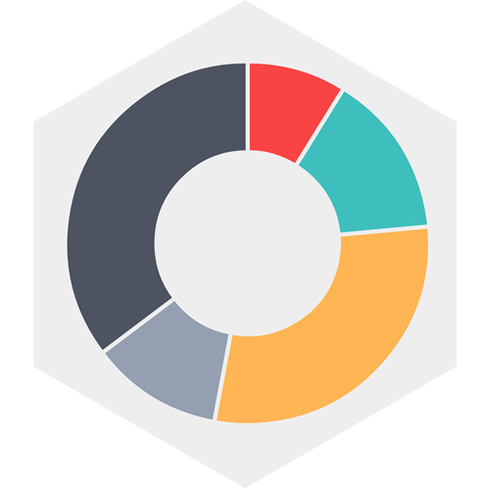
\includegraphics[width=.5\linewidth]{images/chartjs}
%		\captionof{figure}{Chartjs}
%		\label{fig:chartjs-logo}
%    \end{minipage}
%\end{figure}

%\begin{figure}[h]
%	\centering
%	\begin{minipage}{.5\textwidth}
%		\centering
%		
\includegraphics[width=.4\linewidth]{images/npm}
%		\captionof{figure}{npm}
%		\label{fig:npm-logo}
%	\end{minipage}%
%	\begin{minipage}{.5\textwidth}
%		\centering
%		
\includegraphics[width=.4\linewidth]{images/bower}
%		\captionof{figure}{Bower}
%		\label{fig:bower-logo}
%	\end{minipage}
%
%	\begin{minipage}{.5\textwidth}
%		\centering
%		
\includegraphics[width=.5\linewidth]{images/grunt}
%		\captionof{figure}{GruntJs}
%		\label{fig:grunt-logo}
%	\end{minipage}
%\end{figure}

\subsection{Daemon}
The daemon is a python application and can be run only on a linux machine.
Prerequisites
\begin{itemize}
	\item python 3.4+
    \item bluez 5.43+
	\item glib 2
	\item python pip
\end{itemize}
Then you need to clone the repository and configure the MAC address for the smartbands in config/db.json
\begin{lstlisting}[language=Bash]
git clone https://lupu60@bitbucket.org/gnp_team/client-python.git
python3 ClientMain
\end{lstlisting}
%\begin{lstlisting}[language=Bash]
%{
%	"configuration": {
%		"1": {
%			"deviceId": "C8:0F:10:33:A8:3C",
%			"userInfo": {
%				"alias": "Jan",
%				"gender": 1,
%				"weight": 78,
%				"age": 29,
%				"height": 180
%			}
%		}
%	}
%}
%\end{lstlisting}


\section{Toolchain}
In software, a toolchain is a set of programming tools that are used to perform a complex software development task or to create a software product, which is typically another computer program or a set of related programs. In general, the tools forming a toolchain are executed consecutively so the output or resulting environment state of each tool becomes the input or starting environment for the next one, but the term is also used when referring to a set of related tools that are not necessarily executed consecutively.
\newline

First of all the codebase is hosted on bitbucket in a git repository[\footnote{\href{https://lupu60@bitbucket.org/gnp\_team/backend.git}{\texttt{https://lupu60@bitbucket.org/gnp\_team/backend.git}}}], I choose bitbucket because it`s free to host private repository and also for the new feature bitbucket pipelines witch is a continuous delivery system(Figure \ref{fig:piplines}). At a code change on the repository the pipeline will compile my code and deploy to Heroku. In the repository I used the git flow model[\footnote{\href{http://nvie.com/posts/a-successful-git-branching-model/}{\texttt{http://nvie.com/posts/a-successful-git-branching-model/}}}] for the branching strategy.
\begin{figure}[h]
	\centering
	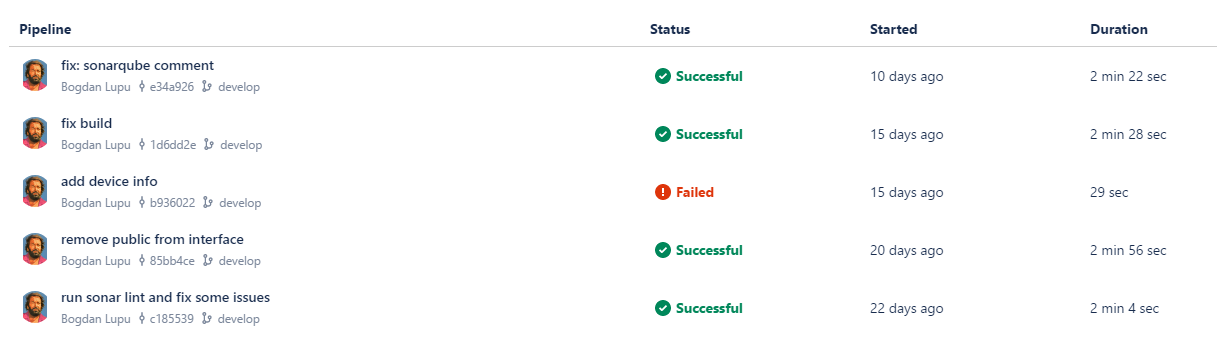
\includegraphics[width=\linewidth]{images/pipelines}
	\caption{Bitbucket Pipelines Dashboard}
	\label{fig:piplines}
\end{figure}

The IoT healtcare has 2 cloud instance a live/production[\footnote{\href{https://iothealthcare.herokuapp.com/}{\texttt{https://iothealthcare.herokuapp.com/}}}] and a prelive/integration [\footnote{\href{https://intiothealthcare.herokuapp.com/}{\texttt{https://intiothealthcare.herokuapp.com/}}}]. This strategy I used is really usefully because I can separate the codebase and not allowing bugs to be on the production. So in the first step I coded local and tested then I push my code to the develop branch form the repository and the bitbucket pipeline will deploy the develop branch on integration and master branch on production, all of this is made it by a bash script. So after I test my code also on the Heroku enviroment I can merge my code from develop to master.
For the code quality I have a sonarQube(Figure \ref{fig:sonar}) instance with docker on my localhost and I run it from time to time.
\begin{figure}[h]
	\centering
	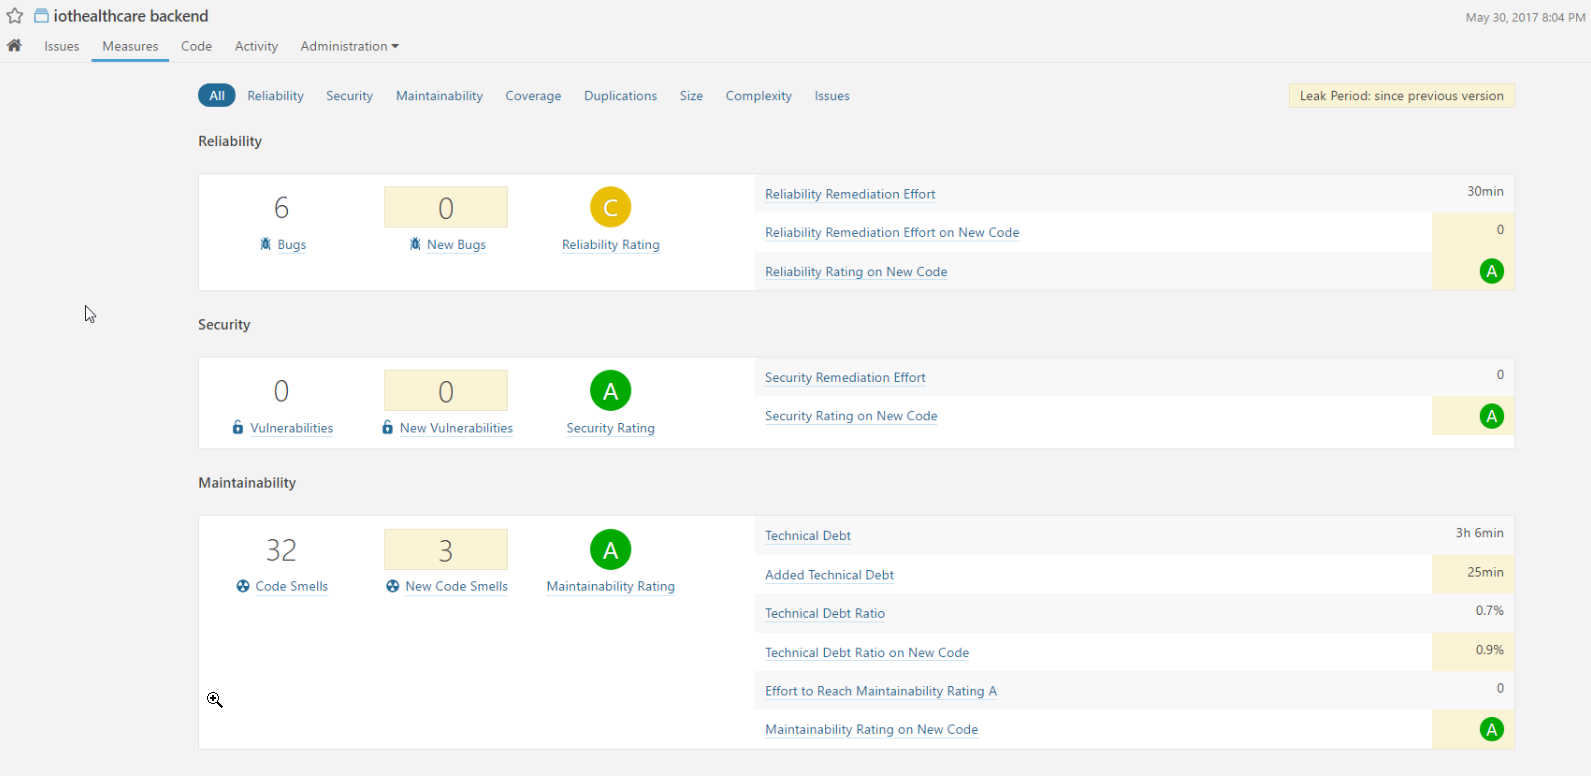
\includegraphics[width=\linewidth]{images/sonarqube}
	\caption{IoT Healthcare: sonarQube build}
	\label{fig:sonar}
\end{figure}
\newline

Now I will present who to run the app and the tools need it.

Necessary installed programs.
\begin{itemize}
	\item Java
	\item nodejs
	\item docker
	\item git
	\item postgreSql (is possible to use a docker image for postgres also)
\end{itemize}
\vspace{5mm}

After you have installed all this programs. First thing we need to do is to clone the repository. So open a command prompt and type the following commands.
\begin{lstlisting}[language=Bash]
git clone https://lupu60@bitbucket.org/gnp_team/backend.git ioth
\end{lstlisting}
\vspace{5mm}

Then configure the database connections properties to connect to the local database in the application.properties file which is located in /src/main/resource.
\begin{lstlisting}[language=Bash]
#localhost POSTGRESQL
spring.datasource.url= jdbc:postgresql://localhost:5432/ioth
spring.datasource.username=postgres
spring.datasource.password=4NzgY09ZdnhZbVir3fUk
\end{lstlisting}
\vspace{5mm}

Now we just need to build the app and start so in the cmd:
\begin{lstlisting}[language=Bash]
cd ioth
npm install -g grunt-cli
npm install -g bower
npm install
gradlew clean build run
\end{lstlisting}
\vspace{5mm}

Access http://localhost:8080/ and the login credentials are user/user. For running the sonarQube you need to install the sonarDocker container and then run the gradlew script but first generate a personal toke form the sonar web interface.
\begin{lstlisting}[language=Bash]
cd ioth
gradlew clean build sonarqube -Dsonar.host.url=http://localhost:<port>
-Dsonar.token=<token>
\end{lstlisting}
\vspace{5mm}

For deploying the app on Heroku after some changes just push the code the default configuration is for the integration, for production open a pull request or merge the develop to master and push.
\begin{lstlisting}[language=Bash]
git checkout master
git pull -r
git merge develop
git push
\end{lstlisting}

For testing the restApi I used postman the postman colletion are avaible in the repostiory in the folder postmanconf.
\begin{figure}[h]
	\centering
	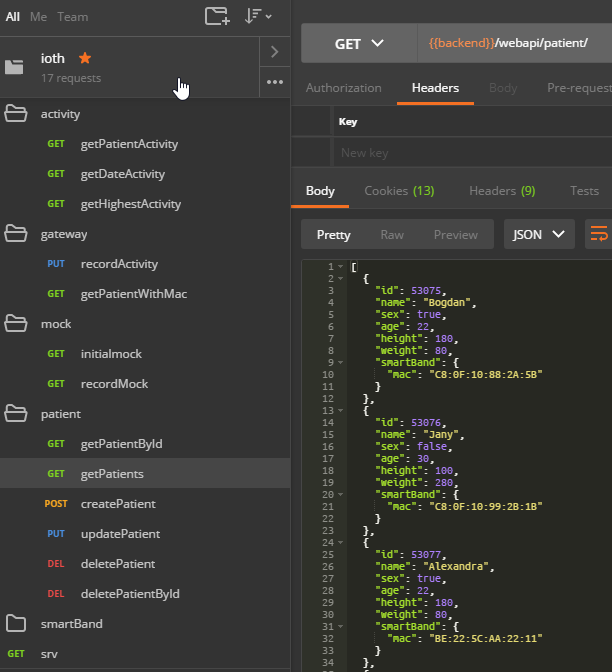
\includegraphics[width=0.7\linewidth]{images/postman}
	\caption{Postman Dashboard}
	\label{fig:postman}
\end{figure}

\section{Tools Used for Development Process}
\subsection{Heroku}
Heroku[\footnote{\href{https://www.heroku.com/home}{\texttt{https://www.heroku.com/home}}}] is a cloud platform as a service (PaaS) supporting several programming languages that is used as a web application deployment model. Heroku, one of the first cloud platforms, has been in development since June 2007, when it supported only the Ruby programming language, but now supports Java, Node.js, Scala, Clojure, Python, PHP, and Go. For this reason, Heroku is said to be a polyglot platform as it lets the developer build, run and scale applications in a similar manner across all the languages. Heroku was acquired by Salesforce.com in 2010 for \$212 million.
\begin{figure}[h!]
	\centering
	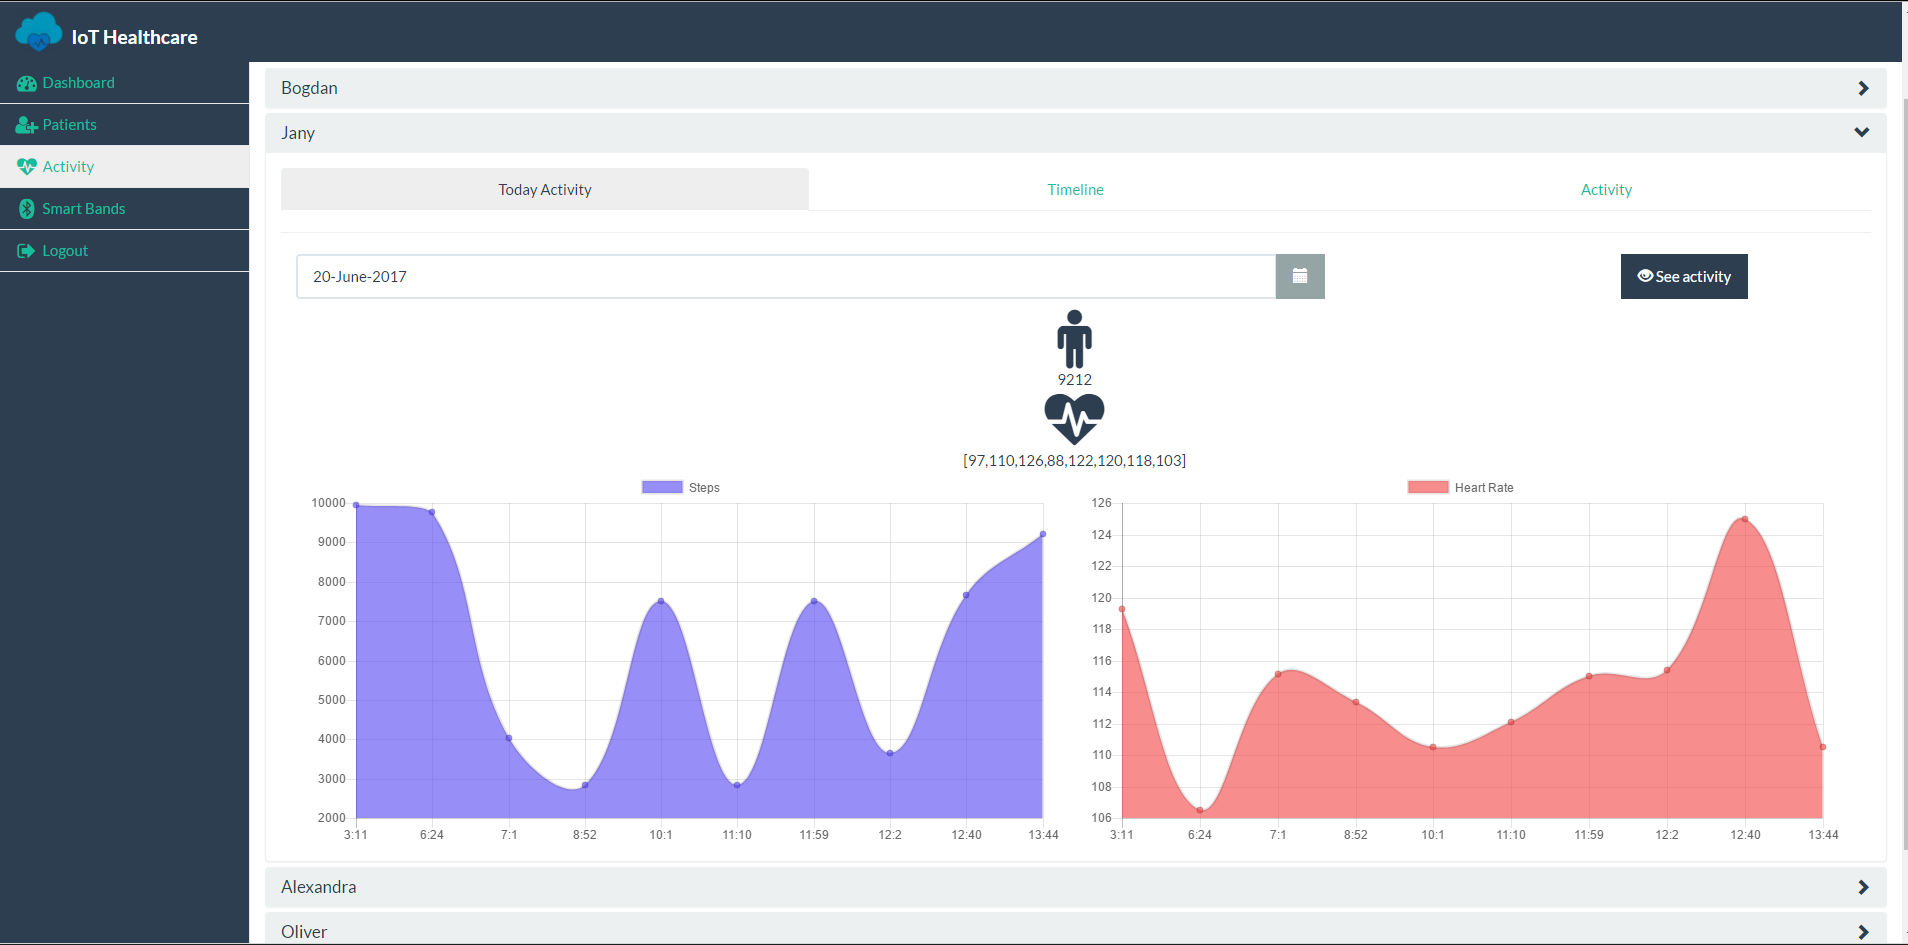
\includegraphics[width=1\textwidth]{./images/iothheroku}
	\rule{1\textwidth}{1pt}
	\caption{IoT Healthcare running on herokucloud}
	\label{fig:iothoh}
\end{figure}
\subsection{Bitbucket}
Bitbucket[\footnote{\href{https://bitbucket.org/}{\texttt{https://bitbucket.org/}}}] is a web-based hosting service that is owned by Atlassian, used for source code and development projects that use either Mercurial (since launch) or Git (since October 2011) revision control systems. Bitbucket offers both commercial plans and free accounts. It offers free accounts with an unlimited number of private repositories (which can have up to five users in the case of free accounts) as of September 2010. Bitbucket integrates with other Atlassian software like Jira, HipChat, Confluence and Bamboo.
It is similar to GitHub, which primarily uses Git. Bitbucket has traditionally tailored itself towards helping professional developers with private proprietary code, especially since being acquired by Atlassian in 2010. In September 2016, Bitbucket announced it had reached 5 million developers and 900,000 teams on its platform.Bitbucket has 3 deployment models: Cloud, Bitbucket Server and Data Center.
\subsection{Sublime Text 2}
Sublime Text 2[\footnote{\href{https://www.sublimetext.com/}{\texttt{https://www.sublimetext.com/}}}] (Figure \ref{fig:sublime}) is the latest version of the popular text editor Sublime Text. It is a full-featured text
editor great for editing local text files. It has many built-in features to aid in editing code, such as
syntax highlighting, auto-indenting, file type recognition, a handy file/folder sidebar for easily
editing of multiple files within a directory, macros to automate repetitious tasks, and tabs and a
split-window option to view and edit multiple files at the same time. With Sublime Text 2's plethora
of programmer-centric features, utilizing this editor can increase your productivity without
bogging you down like full-fledged \textbf{Integrated Development Environments (IDE)} such as \textit{Visual
	Studio} and \textit{Eclipse}. 
\begin{figure}[h!]
	\centering
	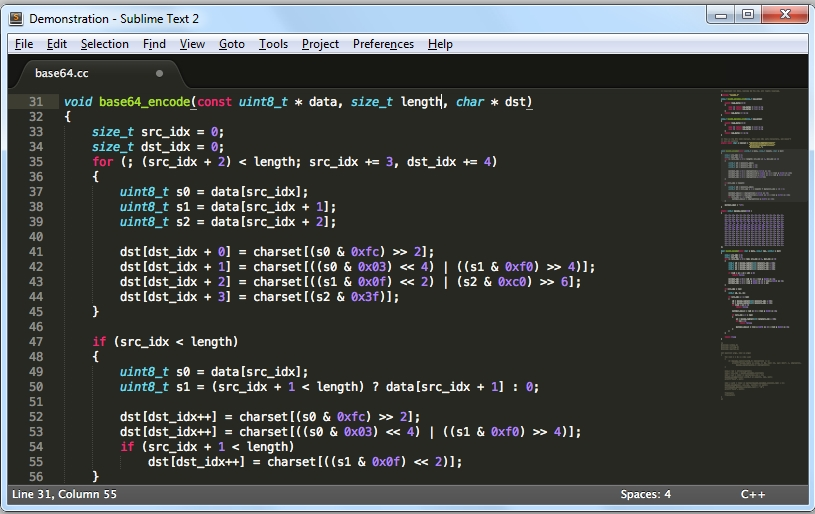
\includegraphics[width=1\textwidth]{./images/sublime.jpg}
	\rule{1\textwidth}{1pt}
	\caption{Sublime Text 2}
	\label{fig:sublime}
\end{figure}

\subsection{Eclipse}
Eclipse (Figure \ref{fig:eclipse}) is an integrated development environment (IDE) used in computer programming, and is the most widely used Java IDE. It contains a base workspace and an extensible plug-in system for customizing the environment. Eclipse is written mostly in Java and its primary use is for developing Java applications, but it may also be used to develop applications in other programming languages via plug-ins, including Ada, ABAP, C, C++, COBOL, D, Fortran, Haskell, JavaScript, Julia, Lasso, Lua, NATURAL, Perl, PHP, Prolog, Python, R, Ruby (including Ruby on Rails framework), Rust, Scala, Clojure, Groovy, Scheme, and Erlang. It can also be used to develop documents with LaTeX (via a TeXlipse plug-in) and packages for the software Mathematica. Development environments include the Eclipse Java development tools (JDT) for Java and Scala, Eclipse CDT for C/C++, and Eclipse PDT for PHP, among others.
\newline
\begin{figure}[h!]
	\centering
	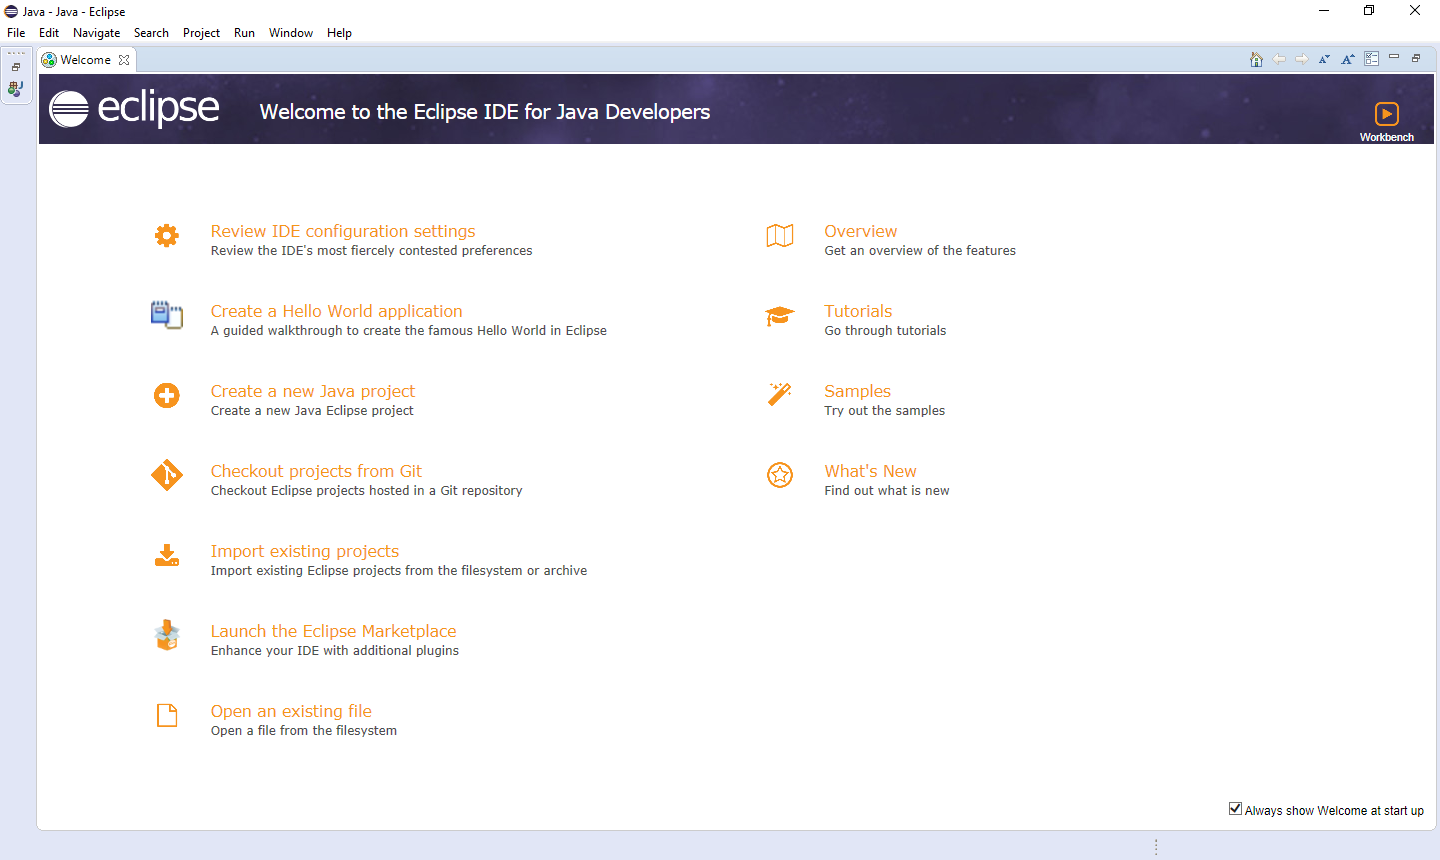
\includegraphics[width=1\textwidth]{./images/eclipse}
	\rule{1\textwidth}{1pt}
	\caption{Eclipse Welcome Screen}
	\label{fig:eclipse}
\end{figure}
The initial codebase originated from IBM VisualAge. The Eclipse software development kit (SDK), which includes the Java development tools, is meant for Java developers. Users can extend its abilities by installing plug-ins written for the Eclipse Platform, such as development toolkits for other programming languages, and can write and contribute their own plug-in modules. Since Equinox, plug-ins can be plugged-stopped dynamically and are termed (OSGI) bundles Eclipse software development kit (SDK) is free and open-source software, released under the terms of the Eclipse Public License, although it is incompatible with the GNU General Public License. It was one of the first IDEs to run under GNU Classpath and it runs without problems under IcedTea.
\subsubsection{PuTTY}
PuTTY (Figure \ref{fig:putty}) is a free and open-source terminal emulator, serial console and network file transfer application. It supports several network protocols, including SCP, SSH, Telnet, rlogin, and raw socket connection. It can also connect to a serial port (since version 0.59). The name "PuTTY" has no definitive meaning.
PuTTY was originally written for Microsoft Windows, but it has been ported to various other operating systems. Official ports are available for some Unix-like platforms, with work-in-progress ports to Classic Mac OS and Mac OS X, and unofficial ports have been contributed to platforms such as Symbian and Windows Mobile.
PuTTY was written and is maintained primarily by Simon Tatham and is currently beta software.
\begin{figure}[h!]
	\centering
	\vspace{-0.2cm}
	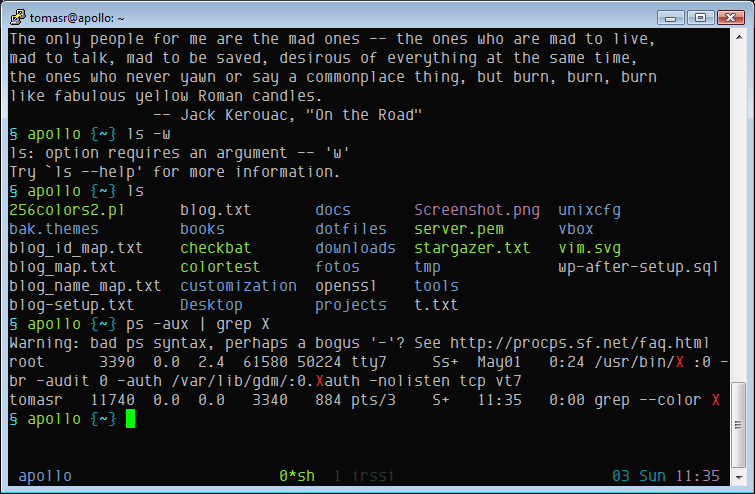
\includegraphics[width=1\textwidth]{./images/putty_tango.png}
	\rule{1\textwidth}{1pt}
	\caption{Putty interface}
	\label{fig:putty}
\end{figure}

%----------------------------------------------------------------------------------------
%	Hardware
%----------------------------------------------------------------------------------------

\section{Hardware}

%-----------------------------------
%	SUBSECTION 1
%-----------------------------------
\subsection{Xiaomi Mi Band}

The Xiaomi Mi Band\footnote{\href{http://www.mi.com/en/miband/}{\texttt{http://www.mi.com/en/miband/}}} (Figure \ref{fig:smartband}) is a wearable fitness tracker produced by Xiaomi. Xiaomi Mi Band was unveiled during a Xiaomi launch event on 22 July 2014.
\begin{figure}[h]
	\centering
	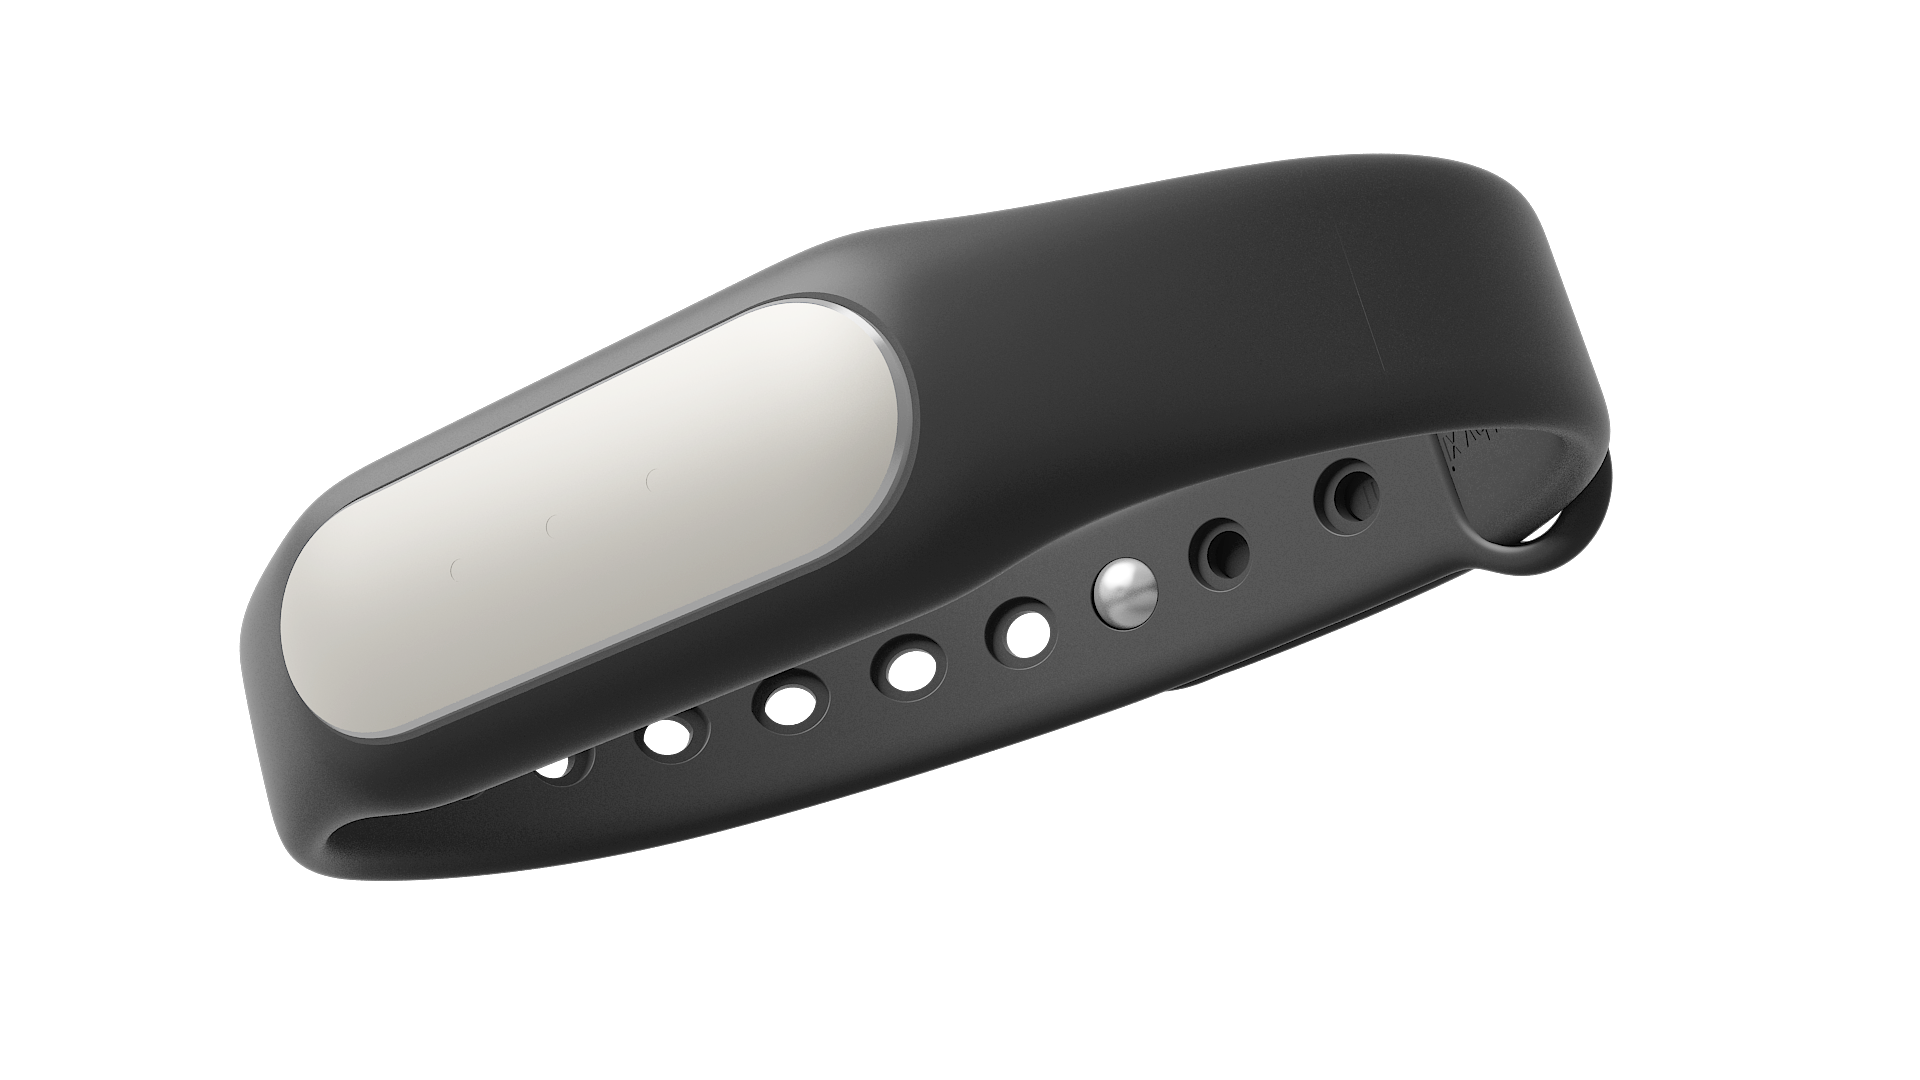
\includegraphics[width=0.7\linewidth]{images/smartband}
	\caption{Xiaomi Mi Band}
	\label{fig:smartband}
\end{figure}

Specifications:
\begin{itemize}
	\item Fitness monitor \& sleep tracker
	\item Sleep-cycle smart alarm
	\item Unlock your Android without a password
	\item 30-day standby power
	\item Water resistant (IP67)
	\item vibrate alert(call \& notification)
\end{itemize}

%-----------------------------------
%	SUBSECTION 2
%-----------------------------------
\subsection{Raspberry Pi}

The Raspberry Pi[\footnote{\href{https://www.raspberrypi.org/help/what-is-a-raspberry-pi/}{\texttt{https://www.raspberrypi.org/help/what-is-a-raspberry-pi/}}}] (Figure \ref{fig:raspberry})  is a series of small single-board computers developed in the United Kingdom by the Raspberry Pi Foundation to promote the teaching of basic computer science in schools and in developing countries. The original model became far more popular than anticipated, selling outside of its target market for uses such as robotics. Peripherals (including keyboards, mice and cases) are not included with the Raspberry Pi. Some accessories however have been included in several official and unofficial bundles.
\begin{figure}[h]
	\centering
	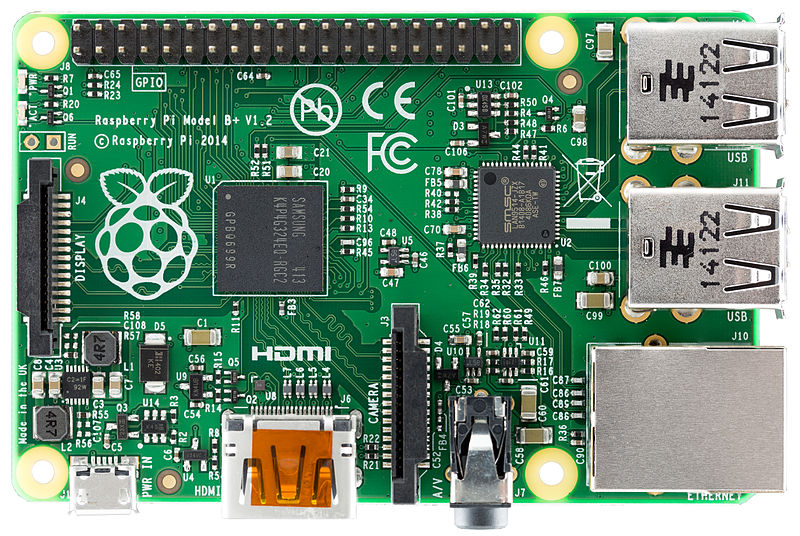
\includegraphics[width=0.5\linewidth]{images/raspberrypi.jpg}
	\caption{Raspberry Pi 1 model B+}
	\label{fig:raspberry}
\end{figure}